\PassOptionsToPackage{table}{xcolor}

% !TEX program = xelatex
\documentclass[aspectratio=169]{beamer}

% =======================
%  COMPILATORE: XeLaTeX
% =======================

% --- Font (Times-like, stabile su Overleaf) ---
\usepackage{fontspec}
\setmainfont{TeX Gyre Termes}
\setsansfont{TeX Gyre Termes}
\setmonofont{TeX Gyre Cursor}

% --- Lingua ---
\usepackage[italian]{babel}

% --- Grafica ---
\usepackage{graphicx}
\usepackage{tikz}
\usetikzlibrary{calc}
\usepackage{media9}
\usepackage{graphicx}

% --- Tema blu ---
\usetheme{Madrid}
%\usecolortheme{default}
\definecolor{TDblue}{RGB}{0,70,140}
\definecolor{TDlight}{RGB}{235,244,252}

\setbeamercolor{structure}{fg=TDblue}
\setbeamercolor{palette primary}{bg=TDblue, fg=white}
\setbeamercolor{frametitle}{bg=TDblue, fg=white}


% \setbeamercolor{structure}{fg=TDblue}
% \setbeamercolor{title}{fg=TDblue}
% \setbeamercolor{frametitle}{fg=TDblue}

\setbeamertemplate{navigation symbols}{}

% =======================
%  Roadmap cliccabile (TOC)
% =======================
\AtBeginSection[]
{
	\begin{frame}{Roadmap}
		\tableofcontents[currentsection, hideallsubsections]
	\end{frame}
}

% =======================
%  Metadati
% =======================
\title[Esperienza 10]{Esperienza 10 — Sensori digitali}
\subtitle{MPU-6050 e test vibrazionale sul modello di un palazzo}
\author{Alessia Di Nino \and Marco Malucchi (T10)}
\date{16 Febbraio 2026}
\institute{TD}

% =======================
%  Helper: box pulito (evita overlay/ombre dei block Madrid)
% =======================
\newcommand{\cleanbox}[2]{%
	\begin{tikzpicture}
		\node[draw=TDblue!70, fill=TDlight, rounded corners=2pt,
		inner xsep=6pt, inner ysep=6pt, align=left, text width=\linewidth] {#2};
	\end{tikzpicture}
}

\usepackage{caption}
\captionsetup[figure]{labelformat=empty}

\begin{document}
	
	% =======================
	%  Prima slide (light, poco testo)
	% =======================
	\begin{frame}[plain]
		\centering
		
		% Immagine in alto al centro
		\vspace*{3mm}
		\IfFileExists{sensore.jpg}{%
			\includegraphics[width=0.36\textwidth]{sensore.jpg}
		}{%
			\fbox{\parbox{0.36\textwidth}{\centering \scriptsize Carica \texttt{sensore.jpg}}}
		}
		
		\vspace{6mm}
		
		{\usebeamerfont{title}\color{TDblue}\Large\textbf{S10 -- Sensori digitali}\par}
		\vspace{3mm}
		
		{\usebeamerfont{subtitle}\normalsize
			MPU-6050 e test vibrazionale sul modello di un palazzo\par}
		
		% niente altro: slide pulita, coerente con “no valanga di testo”
	\end{frame}
	
	% =======================
	%  Roadmap generale
	% =======================
	\begin{frame}{Roadmap}
		\tableofcontents[hideallsubsections]
	\end{frame}
	
	% ==========================================================
	%  SEZIONE 1
	% ==========================================================
	\section{Introduzione e obiettivi}
	
	% ==========================================================
	%  Slide: Introduzione e obiettivi (ridotta + animazioni)
	% ==========================================================
	% ==========================================================
	%  FRAME: CONTESTO (MPU-6050)
	% ==========================================================
	\begin{frame}{Introduzione e Obiettivi}
		
		\begin{columns}[c,onlytextwidth] % 'c' centra verticalmente le colonne tra loro
			
			% ======================
			% COLONNA SINISTRA: TESTO (CENTRATO VERTICALMENTE)
			% ======================
			\begin{column}{0.45\textwidth}
				\centering % Centra il testo orizzontalmente nella colonna
				
				% --- Fase 1: Contesto ---
				\only<1>{
					\textbf{\large Contesto}\\[3mm]
					Il sensore digitale \textbf{MPU-6050} (MEMS) è lo strumento scelto per la \textbf{caratterizzazione dinamica} strutturale.
				}
				
				% --- Fase 2: Obiettivi ---
				\only<2>{
					\textbf{\large Argomenti trattati}\\[3mm]
					{\small
						\begin{itemize}
							\item \textbf{Protocollo}: Comunicazione con MPU-6050 via I$^2$C mediante scrittura diretta dei registri.
							\item \textbf{Analisi Dati}: Validazione statistica e calibrazione.
							\item \textbf{Studio Modale}: Identificazione dei modi normali tramite FFT e fit lorentziani.
						\end{itemize}
					}
				}
			\end{column}
			
			% ======================
			% COLONNA DESTRA: IMMAGINI
			% ======================
			\begin{column}{0.52\textwidth}
				\centering
				
				% Immagine Sensore
				\only<1>{
					\begin{figure}
						\centering
						\IfFileExists{assi.jpg}{
							\includegraphics[width=\linewidth,height=0.7\textheight,keepaspectratio]{assi.jpg}
						}{
							\fbox{\parbox{\linewidth}{\centering \scriptsize [Immagine: \texttt{assi.jpg}]}}
						}
						\caption*{\scriptsize \textit{Sensore}}
					\end{figure}
				}
				
				% Immagine Setup
				\only<2>{
					\begin{figure}
						\centering
						\IfFileExists{setup.jpg}{
							\includegraphics[width=\linewidth,height=0.7\textheight,keepaspectratio]{setup.jpg}
						}{
							\fbox{\parbox{\linewidth}{\centering \scriptsize [Immagine: \texttt{setup.jpg}]}}
						}
						\caption*{\scriptsize \textit{Foto del setup}}
					\end{figure}
				}
			\end{column}
			
		\end{columns}
		
	\end{frame}
	
	
	
	% ==========================================================
	%  SEZIONE 2
	% ==========================================================
	\section{Protocollo di comunicazione I2C.}
	
	\begin{frame}{Architettura digitale: bus I\textsuperscript{2}C}
		
		\begin{columns}[c,onlytextwidth] % [c] garantisce la centratura verticale di entrambe le colonne
			
			% ======================
			% COLONNA SINISTRA: IDEA CHIAVE (TESTO SEMPLICE)
			% ======================
			\begin{column}{0.45\textwidth}
				\uncover<1->{
					\centering
					\textbf{\large Il Principio di Comunicazione}\\[4mm]
					Il dialogo tra microcontrollore e sensore avviene tramite bus \textbf{I\textsuperscript{2}C}: il \textit{Master} interroga periferiche (\textit{Slaves}) univocamente identificate.
				}
			\end{column}
			
			% ======================
			% COLONNA DESTRA: ELEMENTI DEL PROTOCOLLO (BLOCCO)
			% ======================
			\begin{column}{0.50\textwidth}
				\uncover<2->{
					\begin{block}{Architettura del Protocollo}
						\begin{itemize}
							\item \textbf{SDA / SCL}: Linee fisiche di dati e clock.
							\item \textbf{SAD}: Indirizzo univoco del dispositivo.
							\item \textbf{SUB}: Indirizzo del registro interno.
							\item \textbf{ACK}: Validazione della transazione.
						\end{itemize}
					\end{block}
					
					
				}
			\end{column}
			
		\end{columns}
		
	\end{frame}
	
	\begin{frame}{Protocollo I\textsuperscript{2}C: Analisi della Transazione Completa}
		\centering
		
		% 1. Immagine di riferimento superiore (SDA/SCL)
		\uncover<1->{
			\includegraphics[width=0.75\textwidth]{sdascl.png}
			\par\vspace{0.4cm}
		}
		
		% 2. Sequenza animata con nomi file seq1, seq2...
		% Utilizziamo \resizebox per garantire che la riga entri perfettamente nella slide
		\resizebox{\textwidth}{!}{
			\begin{tabular}{@{}c@{\hspace{1pt}}c@{\hspace{1pt}}c@{\hspace{1pt}}c@{\hspace{1pt}}c@{\hspace{1pt}}c@{\hspace{1pt}}c@{\hspace{1pt}}c@{\hspace{1pt}}c@{\hspace{1pt}}c@{\hspace{1pt}}c@{\hspace{1pt}}c@{}}
				\uncover<1->{\includegraphics[height=1.8cm]{seq1.png}} & 
				\uncover<2->{\includegraphics[height=1.8cm]{seq2.png}} & 
				\uncover<3->{\includegraphics[height=1.8cm]{seq3.png}} & 
				\uncover<4->{\includegraphics[height=1.8cm]{seq7.png}} & 
				\uncover<5->{\includegraphics[height=1.8cm]{seq2.png}} & 
				\uncover<6->{\includegraphics[height=1.8cm]{seq6.png}} & 
				\uncover<7->{\includegraphics[height=1.8cm]{seq7.png}} & 
				\uncover<8->{\includegraphics[height=1.8cm]{seq8.png}} & 
				\uncover<9->{\includegraphics[height=1.8cm]{seq9.png}} & 
				\uncover<10->{\includegraphics[height=1.8cm]{seq10.png}} & 
				\uncover<11->{\includegraphics[height=1.8cm]{seq11.png}} & 
				\uncover<12->{\includegraphics[height=1.8cm]{seq12.png}}
			\end{tabular}
		}
		
		\vspace{0.6cm}
		
		% 3. Box di spiegazione dinamica
		\begin{minipage}{0.9\textwidth}
			\setbeamercolor{block body}{bg=TDlight,fg=black}
			\begin{block}{}
				\centering
				\small
				\only<1-4>{Il Master genera lo \textbf{START} e invia il \textbf{SAD (0x68)} + \textbf{Write}. Lo Slave conferma (\textbf{ACK}).}
				\only<5-6>{Viene inviato l'indirizzo del registro interno (\textbf{SUB}) da interrogare. Segue \textbf{ACK}.}
				\only<7-9>{Inizia la lettura: \textbf{Restart} e \textbf{SAD (0x68)} + \textbf{Read} per cambiare direzione ai dati.}
				\only<10-11>{L'MPU-6050 invia il \textbf{Byte di dati}. Il Master chiude con \textbf{NACK} (o ACK se continua).}
				\only<12>{La transazione termina con la condizione di \textbf{STOP}, liberando le linee SDA/SCL.}
			\end{block}
		\end{minipage}
		
	\end{frame}
	
	% ==========================================================
	%  SEZIONE 3
	% ==========================================================
	\section{Caratteristiche di MPU-6050.}
	
	% ==========================================================
	% SLIDE 1: Architettura Interna e Flusso Dati
	% ==========================================================
	\begin{frame}{Architettura dell'MPU-6050}
		\begin{columns}[c,onlytextwidth]
			
			% Colonna Sinistra (1/3)
			\begin{column}{0.30\textwidth}
				% \begin{block}{Il Dispositivo}
					%   \textbf{3 Assi}: 
					%   \begin{itemize}
						%       \item 3 Accelerazioni 
						%       \item 3 Velocità angolari
						%   \end{itemize}
					%   \vspace{2mm}
					%   \textbf{Pin Essenziali}: \\ 
					%   VDD, GND, SDA, SCL.
					% \end{block}
				
				% \vspace{4mm}
				% \centering
				% \IfFileExists{collegamenti_pin.jpg}{
					%   \includegraphics[width=0.6\linewidth]{collegamenti_pin.jpg}
					% }{
					%   \fbox{\scriptsize Foto moduli}
					% }
				\begin{itemize}
					\item Circuitria del sensore
					\item Blocco di trasduzione
					\item Blocco di controllo e gestione della comunicazione I$^2$C
				\end{itemize}
			\end{column}
			
			% Colonna Destra (2/3) - Animazione Diagrammi
			\begin{column}{0.65\textwidth}
				\centering
				\only<1>{
					\IfFileExists{block_diagram.png}{
						\includegraphics[width=\linewidth,height=0.7\textheight,keepaspectratio]{block_diagram.png}
					}{
						\fbox{\parbox{0.8\linewidth}{\centering \scriptsize [Carica block\_diagram.png]}}
					}
					\par\vspace{2mm}{\scriptsize \textit{Architettura funzionale dei registri e sensori}}
				}
				% \only<2>{
					%   \IfFileExists{block_diagram_FIFO.png}{
						%     \includegraphics[width=\linewidth,height=0.7\textheight,keepaspectratio]{block_diagram_FIFO.png}
						%   }{
						%     \fbox{\parbox{0.8\linewidth}{\centering \scriptsize [Carica block\_diagram\_FIFO.png]}}
						%   }
					%   \par\vspace{2mm}{\scriptsize \textit{Gestione del buffer FIFO per il campionamento sincrono}}
					% }
			\end{column}
		\end{columns}
	\end{frame}
	
	% ==========================================================
	%  SEZIONE 4
	% ==========================================================
	\section{Studio statistico del sensore.}
	% ==========================================================
	%  Slide: Studio statistico (Task 6)
	%  Richiede i file:
	%   - andamento_medie.png
	%   - andamento_std-dev.png
	% ==========================================================
	\begin{frame}{Caratterizzazione Statistica del Rumore}
		
		% --- 1. Analisi Preliminare a tutto schermo ---
		\only<1>{
			\begin{figure}
				\centering
				\includegraphics[width=\textwidth,height=0.8\textheight,keepaspectratio]{fit_gaussiano_preliminare.png}
				\vspace{-0.2cm}
				\caption{\scriptsize Serie temporali e istogrammi campionari}
			\end{figure}
		}
		
		% --- 2. Modello Matematico ---
		\only<2-4>{
			\centering
			\vspace{0.5cm}
			{\Large \textbf{Modello di Fit: Gaussian Bin Integral}} \\
			\vspace{0.8cm}
			
			% Click 2
			\uncover<2->{Non si è optato per una distribuzione gaussina semplice come modello di fit, bensì si è deciso di integrare la gaussiana sulla larghezza del bin, detta $\Delta$:}
			
			% Click 3
			\uncover<3->{
				$$f(x_c) = \int_{x_c - \frac{\Delta}{2}}^{x_c + \frac{\Delta}{2}} \frac{N}{\sqrt{2\pi\sigma^2}} e^{-\frac{(t-\mu)^2}{2\sigma^2}} dt$$
			}
			
			% Click 4 (La formula finale appare subito dopo l'integrale)
			\uncover<4->{
				$$f(x_c) = \frac{N}{2} \left[ \text{erf}\left( \frac{x_c + \frac{\Delta}{2} - \mu}{\sqrt{2}\sigma} \right) - \text{erf}\left( \frac{x_c - \frac{\Delta}{2} - \mu}{\sqrt{2}\sigma} \right) \right]$$
			}
		}
		
		% --- 3. Fit Residui a tutto schermo ---
		% Inizia dal click 5
		\only<5>{
			\begin{figure}
				\centering
				\includegraphics[width=\textwidth,height=0.8\textheight,keepaspectratio]{fit_gaussiano_residui.png}
				\vspace{-0.2cm}
				\caption{\scriptsize Analisi dei residui e $\tilde{\chi}^2$}
			\end{figure}
		}
		
		% --- 4. Fit Residui rimpicciolito + Tabella ---
		% Click 6
		\only<6>{
			\begin{columns}[c]
				\begin{column}{0.65\textwidth}
					\begin{figure}
						\centering
						\includegraphics[width=\textwidth]{fit_gaussiano_residui.png}
						\caption{\scriptsize Analisi dei residui e $\tilde{\chi}^2$}
					\end{figure}
				\end{column}
				
				\begin{column}{0.35\textwidth}
					\centering
					\footnotesize
					\textbf{Risultati Finali} \\
					\vspace{0.2cm}
					\begin{tabular}{|l|}
						\hline
						\rowcolor{TDlight} \textbf{Asse X} \\ \hline
						$\mu = (6.515 \pm 0.006) \cdot 10^{-2}$ g \\
						$\sigma = (1.461 \pm 0.004) \cdot 10^{-3}$ g \\ \hline
						\hline
						\rowcolor{TDlight} \textbf{Asse Y} \\ \hline
						$\mu = (1.782 \pm 0.006) \cdot 10^{-2}$ g \\
						$\sigma = (1.407 \pm 0.004) \cdot 10^{-3}$ g \\ \hline
					\end{tabular}
				\end{column}
			\end{columns}
		}
	\end{frame}
	
	
	% ==========================================================
	%  SEZIONE 5
	% ==========================================================
	\section{Esperimento: modello di palazzo}
	
	
	\begin{frame}
		% --- Titolo (sempre presente) ---
		\begin{center}
			\Large \bfseries  
			Test vibrazionale di un modello che replica la \\ 
			struttura di un palazzo a due piani
			\vspace{0.4cm}
			\hrule height 1pt
		\end{center}
		
		% --- FASE 1: Immagini sequenziali e Obiettivi (Click 1-6) ---
		\only<1-6>{
			\begin{columns}[T]
				\begin{column}{0.65\textwidth}
					\centering \vspace{0.2cm}
					\only<2>{\includegraphics[width=\textwidth,height=0.7\textheight,keepaspectratio]{modello_masse1.jpg}}
					\only<3>{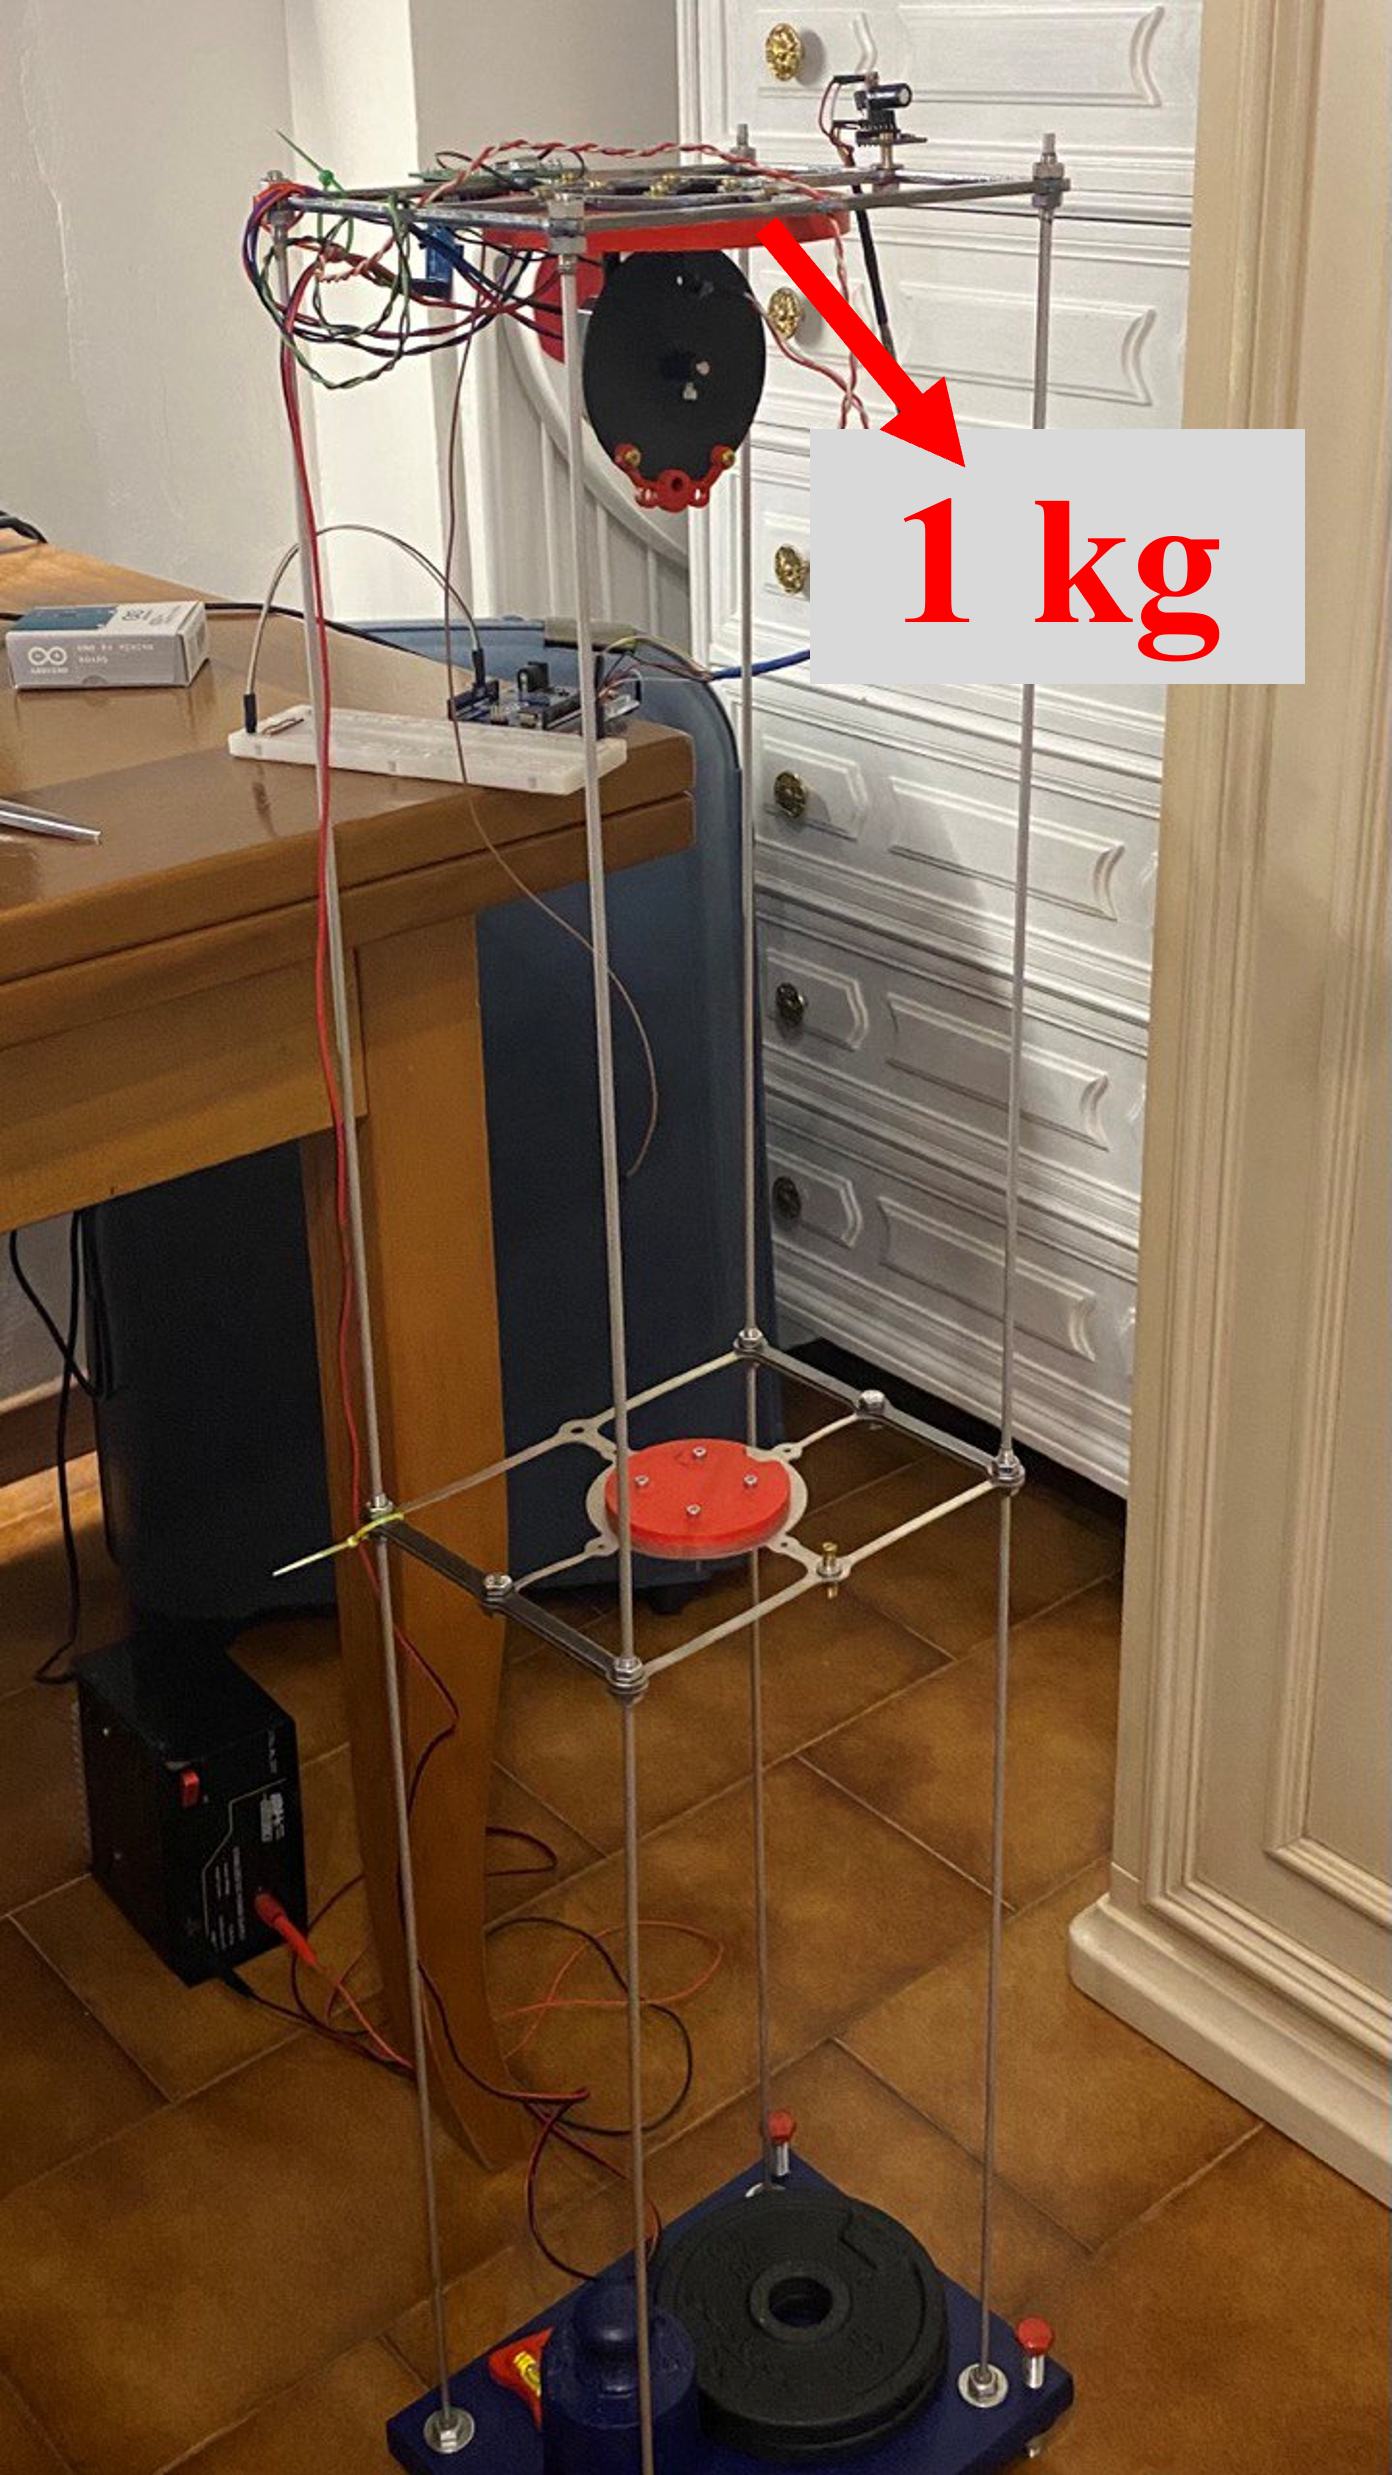
\includegraphics[width=\textwidth,height=0.7\textheight,keepaspectratio]{modello_masse2.png}}
					\only<4>{\includegraphics[width=\textwidth,height=0.7\textheight,keepaspectratio]{modello_masse3.png}}
					\only<5-6>{\includegraphics[width=\textwidth,height=0.7\textheight,keepaspectratio]{modello_masse4.png}}
				\end{column}
				
				\begin{column}{0.35\textwidth}
					\uncover<6>{
						\vspace{1.5cm}
						{\large \bfseries Obiettivi:} \vspace{0.5cm}
						\begin{itemize}
							\item[\textbullet] Test vibrazionale \vspace{0.3cm}
							\item[\textbullet] Analisi modale
						\end{itemize}
					}
				\end{column}
			\end{columns}
		}
		
		% --- FASE 2: Layout in tre parti (Click 7) ---
		\only<7>{
			\begin{columns}[T]
				% 1/3: Vecchia foto rimpicciolita
				\begin{column}{0.33\textwidth}
					\centering \vspace{0.5cm}
					\includegraphics[width=\textwidth,height=0.6\textheight,keepaspectratio]{modello_masse4.png}
					\captionof{figure}{\scriptsize Setup Struttura}
				\end{column}
				
				% 2/3: Nuova foto Impulse
				\begin{column}{0.33\textwidth}
					\centering \vspace{0.5cm}
					\includegraphics[width=\textwidth,height=0.6\textheight,keepaspectratio]{impulse.jpg}
					\captionof{figure}{\scriptsize Stimolo Impulsivo}
				\end{column}
				
				% 3/3: Testo Metodologia
				\begin{column}{0.33\textwidth}
					\vspace{1cm}
					\textbf{ Metodologia Sperimentale}
					\begin{itemize}
						\item Pendolo semplice per stimolo impulsivo ($\delta$).
						\item Acquisizione della risposta temporale.
					\end{itemize}
					\vspace{0.3cm}
					\textbf{Analisi Modale}
					\begin{itemize}
						\item Identificazione risonanze dai picchi di $|H(\omega)|$.
					\end{itemize}
				\end{column}
			\end{columns}
		}
	\end{frame}
	
	\begin{frame}{Analisi in Frequenza: Power Spectral Density (PSD)}
		\begin{columns}[T]
			% --- Colonna Sinistra (2/3): Immagini a scorrimento ---
			\begin{column}{0.66\textwidth}
				\centering
				\vspace{0.2cm}
				% Ogni immagine appare al click corrispondente e scompare per la successiva
				\only<1>{\includegraphics[width=\textwidth,height=0.7\textheight,keepaspectratio]{PSD_mediato_altax.png}}
				\only<2>{\includegraphics[width=\textwidth,height=0.7\textheight,keepaspectratio]{PSD_mediato_altay.png}}
				\only<3>{\includegraphics[width=\textwidth,height=0.7\textheight,keepaspectratio]{PSD_mediato_alta_ruotato.png}}
				\only<4>{\includegraphics[width=\textwidth,height=0.7\textheight,keepaspectratio]{PSD_mediato_bassay.png}}
				
				\captionof{figure}{\scriptsize 
					\only<1>{Perturbazione Parte Alta - Lungo X}
					\only<2>{Perturbazione Parte Alta - Lungo Y}
					\only<3>{Perturbazione Parte Alta - Ruotata}
					\only<4>{Perturbazione Parte Bassa - Lungo X}
				}
			\end{column}
			
			% --- Colonna Destra (1/3): Testo fisso ---
			\begin{column}{0.33\textwidth}
				\vspace{1cm}
				\begin{itemize}
					\item Passaggio in trasformata
					\vspace{0.4cm}
					\item Analisi di 4 perturbazioni:
					\begin{itemize}
						\item[\tiny\textbullet] Parte alta: $x, y$, ruotata.
						\item[\tiny\textbullet] Parte bassa: solo lungo $x$.
					\end{itemize}
					\vspace{0.4cm}
					\item Ogni spettro rappresenta la \textbf{PSD mediata su 10 acquisizioni} per ridurre il rumore.
				\end{itemize}
			\end{column}
		\end{columns}
	\end{frame}
	
	% ==========================================================
	%  SLIDE ZOOM (Senza fascia blu, 4 immagini a tutto schermo)
	% ==========================================================
	% ==========================================================
	\begin{frame}[plain]
		\centering
		
		% --- Click 1: Grid dei 4 Zoom ---
		\only<1>{
			\vspace*{0.1cm}
			\begin{columns}[onlytextwidth]
				\begin{column}{0.49\textwidth}
					\centering
					\includegraphics[width=\linewidth,height=0.46\textheight,keepaspectratio]{PSD_mediato_altax_zoom.png}
				\end{column}
				\begin{column}{0.49\textwidth}
					\centering
					\includegraphics[width=\linewidth,height=0.46\textheight,keepaspectratio]{PSD_mediato_altay_zoom.png}
				\end{column}
			\end{columns}
			\vspace{0.2cm}
			\begin{columns}[onlytextwidth]
				\begin{column}{0.49\textwidth}
					\centering
					\includegraphics[width=\linewidth,height=0.46\textheight,keepaspectratio]{PSD_mediato_alta_ruotato_zoom.png}
				\end{column}
				\begin{column}{0.49\textwidth}
					\centering
					\includegraphics[width=\linewidth,height=0.46\textheight,keepaspectratio]{PSD_mediato_bassay_zoom.png}
				\end{column}
			\end{columns}
		}
		
		% --- Click 2: Picchi ---
		\only<2>{
			\includegraphics[width=0.9\paperwidth,height=\paperheight,keepaspectratio]{picchi.png}
		}
		
		% --- Click 3: Fase meno rilevante ---
		\only<3>{
			\includegraphics[width=0.9\paperwidth,height=\paperheight,keepaspectratio]{fase_meno_rilevante.png}
		}
		
		% --- Click 4: Fase rilevante ruotato ---
		\only<4>{
			\includegraphics[width=0.9\paperwidth,height=\paperheight,keepaspectratio]{picchetti_ipotesi.png}
		}
		
		% --- Click 5: Picchetti ipotesi ---
		\only<5>{
			\includegraphics[width=0.9\paperwidth,height=\paperheight,keepaspectratio]{fase_rilevante_ruotato.png}
		}
		
		% --- Click 6: Analisi Modi Torsionali ---
		\only<6>{
			\includegraphics[width=0.9\textwidth,height=\paperheight,keepaspectratio]{torsionali_bene.png}
		}
		
		% --- Click 7: Analisi Modi in Controfase ---
		\only<7>{
			\includegraphics[width=0.9\textwidth,height=\paperheight,keepaspectratio]{controfase_bene.png}
		}
	\end{frame}
	
	\begin{frame}{Analisi delle Acquisizioni: Fit Lorentziani}
		
		% --- Overlay 1: Teoria e Metodologia ---
		\only<1>{
			\centering
			\textbf{Modello di Fit: Lorentziane multiple} \\
			\vspace{0.2cm}
			$$L(f) = \sum_{i} \frac{A_i}{1 + \left( \frac{f - f_{0,i}}{\gamma_i} \right)^2}$$
			\vspace{0.4cm}
			\begin{columns}[T]
				\begin{column}{0.5\textwidth}
					\begin{itemize}
						\item[\textbullet] \textbf{Approccio analitico:} Identificazione dei picchi.
						\item[\textbullet] \textbf{Boundaries:} Vincoli su $f_0$ ($\pm 0.5$ Hz) e $\gamma$ ($[0.001, 5]$) per garantire la convergenza fisica del fit.
						\item[\textbullet] \textbf{Soglia:} Trascurati picchi sotto $5 \cdot 10^{-3}$ $\mathrm{g^2/Hz}$ (con tolleranza adattiva).
					\end{itemize}
				\end{column}
				\begin{column}{0.5\textwidth}
					\begin{itemize}
						\item[\textbullet] \textbf{Medie Pesate:} Calcolate con pesi $w_i = 1/\sigma_i^2$.
						\item[\textbullet] \textbf{Validità:} Analisi limitata al range $[0.5, 20]$ Hz per escludere offset DC e rumore ad alta frequenza.
					\end{itemize}
				\end{column}
			\end{columns}
		}
		
		% --- Overlay 2: Risultati Alta Y ---
		\only<2>{
			\begin{columns}[c]
				\begin{column}{0.55\textwidth}
					\includegraphics[width=\textwidth]{fit_combined_pres_altay.png}
				\end{column}
				\begin{column}{0.45\textwidth}
					\scriptsize
					\textbf{Fit Parte Alta (Asse Y) - Parametri Chiave}
					\begin{itemize}
						\item \textbf{Fase:} $f_0 \approx 1.70$ Hz | $Q \approx 115$
						\item \textbf{Controfase:} $f_0 \approx 4.75$ Hz | $Q \approx 45$
						\item \textbf{Torsionale controfase:} $f_0 \approx 15.26$ Hz | $Q \approx 39$
					\end{itemize}
					\vspace{0.3cm}
					\includegraphics[width=\textwidth]{linear_residuals_pres_altay.png}
				\end{column}
			\end{columns}
		}
		
		% --- Overlay 3: Risultati Bassa X ---
		\only<3>{
			\begin{columns}[c]
				\begin{column}{0.55\textwidth}
					\includegraphics[width=\textwidth]{fit_combined_pres_bassax.png}
				\end{column}
				\begin{column}{0.45\textwidth}
					\scriptsize
					\textbf{Fit Parte Bassa (Asse X) - Parametri Chiave}
					\begin{itemize}
						\item \textbf{Controfase:} $f_0 \approx 5.84$ Hz | $Q \approx 108$
					\end{itemize}
					\vspace{0.3cm}
					\includegraphics[width=\textwidth]{linear_residuals_pres_bassax.png}
				\end{column}
			\end{columns}
		}
		
		% --- Overlay 4: Tabellona Finale (Centrata) ---
		\only<4>{
			\begin{columns}[c] % Centratura verticale
				\begin{column}{0.65\textwidth}
					\centering
					\scriptsize
					\textbf{Riepilogo Parametri di fit} \\
					\vspace{0.2cm}
					\begin{tabular}{l|l|c|c|c}
						\hline
						\textbf{Configurazione} & \textbf{Modo (asse)} & $f_0$ [Hz] & $\gamma$ [Hz] & $Q$ Factor \\ \hline
						% Parte Alta X
						Parte Alta X & Fase (X) & $0.900 \pm 0.003$ & $0.017 \pm 0.002$ & $27 \pm 3$ \\
						Parte Alta X & Tor fase (Y) & $4.64 \pm 0.01$ & $0.10 \pm 0.01$ & $23 \pm 3$ \\
						Parte Alta X & Tor contro (Y) & $15.24 \pm 0.02$ & $0.20 \pm 0.02$ & $38 \pm 3$ \\ \hline
						% Parte Alta Y
						Parte Alta Y & Fase (X) & $0.86 \pm 0.01$ & $0.01 \pm 0.02$ & $40 \pm 70$ \\
						Parte Alta Y & Controfase (X) & $5.84 \pm 0.01$ & $0.08 \pm 0.01$ & $37 \pm 5$ \\
						Parte Alta Y & Fase (Y) & $1.698 \pm 0.003$ & $0.007 \pm 0.007$ & $115 \pm 112$ \\
						Parte Alta Y & Tor fase (Y) & $4.751 \pm 0.007$ & $0.053 \pm 0.007$ & $45 \pm 6$ \\
						Parte Alta Y & Tor contro (Y) & $15.26 \pm 0.01$ & $0.20 \pm 0.01$ & $39 \pm 3$ \\ \hline
						% Parte Bassa Y
						Parte Bassa & Controfase (X) & $5.84 \pm 0.01$ & $0.03 \pm 0.02$ & $108 \pm 60$ \\
						Parte Bassa & Controfase (Y) & $5.786 \pm 0.008$ & $0.06 \pm 0.01$ & $49 \pm 9$ \\
						Parte Bassa & Tor contro (Y) & $14.93 \pm 0.04$ & $0.22 \pm 0.03$ & $34 \pm 5$ \\ \hline
						% Ruotato
						Ruotato & Fase (X) & $0.873 \pm 0.004$ & $0.007 \pm 0.004$ & $63 \pm 32$ \\
						Ruotato & Fase (Y) & $1.750 \pm 0.006$ & $0.010 \pm 0.007$ & $86 \pm 56$ \\
						Ruotato & Tor fase (Y) & $4.73 \pm 0.01$ & $0.07 \pm 0.01$ & $33 \pm 7$ \\ \hline
					\end{tabular}
				\end{column}
				\begin{column}{0.25\textwidth}
					\scriptsize
					\textbf{Osservazioni Finali:}
					\begin{itemize}
						\item[\textbullet] \textbf{Inconsistenza Statistica:} $\chi^2_{red} < 1$ suggerisce una sovrastima delle incertezze.
						\item[\textbullet] \textbf{Stabilità:} Risultati qualitativamente consistenti tra i diversi set di acquisizione.
						\item[\textbullet] \textbf{Dissipazione:} I modi torsionali mostrano un damping rate $\gamma$ più elevato.
						\item[\textbullet] \textbf{Q-Factor:} Minore per i modi torsionali, confermando una dissipazione energetica più accentuata rispetto agli altri modi di oscillazione.
					\end{itemize}
				\end{column}
			\end{columns}
		}
	\end{frame}
	
	\begin{frame}{Transizione: Dalle Oscillazioni Libere alla Risposta Forzata}
		\centering
		\textbf{Limiti dell'Analisi Stocastica} \\
		\vspace{0.2cm}
		\begin{itemize}
			\item \textbf{Segnale rumoroso:} Nonostante la media su $N=10$, il rumore di fondo rimane una componente critica.
			\item \textbf{Scarsa ripetibilità:} La risoluzione dei parametri dipende dall'eccitazione ambientale casuale.
		\end{itemize}
		
		\vspace{0.4cm}
		\hrule
		\vspace{0.4cm}
		
		\textbf{Prossima Fase: Spazzata in Frequenza} \\
		\vspace{0.2cm}
		\begin{itemize}
			\item \textbf{Range di indagine:} Analisi in frequenza tra 0.5 Hz e 15.7 Hz.
			\item \textbf{Strategia di campionamento:}
			\begin{itemize}
				\item Risoluzione larga di $1/10$ Hz per la scansione generale.
				\item Risoluzione fine di $2/100$ Hz in prossimità dei picchi
			\end{itemize}
			\item \textbf{Parametri di output:} Caratterizzazione tramite \textbf{Guadagno} e \textbf{Sfasamento}.
		\end{itemize}
		
		
	\end{frame}
	
	\begin{frame}{Analisi Modale: acquisizioni delle spazzate in frequenza.}
		
		\only<1>{
			\begin{figure}
				\centering
				\includegraphics[width=\textwidth,height=0.8\textheight,keepaspectratio]{spazzata_completa_x_modulo.png}
			\end{figure}
		}
		
		\only<2>{
			\begin{figure}
				\centering
				\includegraphics[width=\textwidth,height=0.8\textheight,keepaspectratio]{spazzata_completa_x_fase.png}
			\end{figure}
		}
		
		
		\only<3>{
			\begin{columns}[T]
				% --- Colonna Sinistra: Immagini grandi ---
				\begin{column}{0.5\textwidth}
					\begin{figure}
						\centering
						\includegraphics[width=\textwidth]{spazzata_completa_y_modulo.png}
						\caption{\scriptsize Guadagno asse y}
					\end{figure}
				\end{column}
				
				% --- Colonna Destra: Obiettivi puliti ---
				\begin{column}{0.5\textwidth}
					\begin{figure}
						\centering
						\includegraphics[width=\textwidth]{spazzata_completa_y_fase.png}
						\caption{\scriptsize Sfasamento asse y}
					\end{figure}
				\end{column}
			\end{columns}
		}
		
	\end{frame}
	
	\begin{frame}{Analisi Modale: modello teorico.}
		\only<1-4>{
			\begin{itemize}
				\item<1-> Picchi asimmetrici $\Rightarrow$ modello \textbf{non} Lorentziano per singoli picchi.
				\item<2-> Il sistema può essere interpretato come \textbf{oscillatore a più gradi di libertà} (sistema MDOF).
				\item<3-> "Dip" tra un picco ed il successivo indicano \textbf{antirisonanze} ed \textbf{interazione tra i modi normali} della struttura.
				\item<4->[] $\Rightarrow$ \textbf{interferenza tra i modi normali della struttura}.
			\end{itemize}
		}
		
		\uncover<5-7>{
			\begin{itemize}
				\item<5-> Il sistema è MDOF, ogni modo è modellizzabile come \textbf{oscillatore armonico smorzato}
				\item<6-> Globalmente ho una somma di funzioni di trasferimento di singoli oscillatori smorzati:
				\begin{equation}
					H(\omega) = \sum_{k=1}^{n} H_k(\omega) = \sum_{k=1}^{n}\frac{R_k}{\omega_k^2 - \omega^2 + i\,2\zeta_k \omega_k \omega}
					\label{FRF}
				\end{equation}
				\only<7>{
					\item $\omega_k$ frequenza del modo k-esimo.
					\item $\zeta_k$ tasso di smorzamento.
					\item $R_k$ importanza del modo k-esimo nella dinamica globale.
				}
			\end{itemize}	
		}
	\end{frame}
	
	\begin{frame}{Fit delle spazzate.}
		\only<1>{
			\begin{itemize}
				\item Scelgo come modello di fit \eqref{FRF}, moltiplicato per $\omega^2$, poiché i dati misurati sono delle \textbf{accelerazioni}:
				\[
				H(\omega) = \frac{\tilde{X}(\omega)}{\tilde{f}(\omega)} \; ; \; \tilde{a}(\omega) = \omega^2 \tilde{X}(\omega)
				\]
				fitto 
				\[\frac{\tilde{a}}{\tilde{f}} = \omega^2 H(\omega)\]
				dove $f = r \omega^2$ accelerazione centrifuga su massa fuori asse della vibrodina
			\end{itemize}
		}
		
		\only<2>{
			\begin{figure}
				\centering
				\includegraphics[width=\textwidth,height=1\textheight,keepaspectratio]{simulazione_1.png}
			\end{figure}		
		}
		
		\only<3>{
			\begin{figure}
				\centering
				\includegraphics[width=\textwidth,height=0.8\textheight,keepaspectratio]{FIT_AMPIEZZA_X.png}
			\end{figure}
		}
		
		\only<4>{
			\begin{figure}
				\centering
				\includegraphics[width=\textwidth,height=0.8\textheight,keepaspectratio]{FIT_FASE_X.png}
			\end{figure}
		}
		
		\only<5>{
			\begin{table}
				\centering
				\small
				\begin{tabular}{c c c c c}
					\hline
					\textbf{Modo} & $f_k$ (Hz) & $R_k$ & $\zeta_k$ & $Q_k$ \\
					\hline
					
					1 & $0.88808 \pm 0.00001$
					& $(9.44 \pm 0.02)\times10^{-4}$
					& $(3.09 \pm 0.09)\times10^{-3}$
					& $162 \pm 5$ \\
					
					2 & $4.7418 \pm 0.0004$
					& $(3.39 \pm 0.07)\times10^{-5}$
					& $(6.31 \pm 0.09)\times10^{-3}$
					& $79 \pm 1$ \\
					
					3 & $5.8127 \pm 0.0001$
					& $(1.238 \pm 0.004)\times10^{-4}$
					& $(4.99 \pm 0.02)\times10^{-3}$
					& $100.1 \pm 0.5$ \\
					
					4 & $14.6 \pm 0.01$
					& $(8 \pm 1)\times10^{-6}$
					& $(4.4 \pm 0.2)\times10^{-2}$
					& $11.3 \pm 0.5$ \\
					
					\hline
				\end{tabular}
				\caption{Parametri di best fit per spazzata asse X mediati tra fit guadagno e sfasamento.}
			\end{table}
			
		}
		
	\end{frame}
	
	% ==========================================================
	%  SEZIONE 6
	% ==========================================================
	\section{Conclusioni e prospettive}
	\begin{frame}{Conclusioni: fit non buoni.}
			\begin{itemize}
				\item Chi quadro ridotto \textbf{sistematicamente troppo basso o troppo alto}.
				\item Valori parametri di best fit hanno \textbf{accordo qualitativo}.
				\item[] $\Rightarrow$ I risultati ottenuti hanno \textbf{scarsa significatività statistica}
			\end{itemize}
	\end{frame}
	
	\begin{frame}{Conclusioni: veridicità dei risultati.}
			\begin{itemize}
				\item Resta la ragionevolezza dei risultati.
				\item \textbf{Il modello è corretto}.
				\item[] $\Rightarrow$ \textbf{Interpretazione fisica corretta}.
				\item Risultati in \textbf{accordo qualitativo con osservazioni sperimentali}.
				\item Altre caratteristiche fisiche deducibili dai parametri.
			\end{itemize}
	\end{frame}
	
	\begin{frame}{Conclusioni: problema.}
			\begin{itemize}
				\item Allora dov'è il problema?
				\item[] $\Rightarrow$ \textbf{Incertezze} sulle misure \textbf{non correttamente stimate}.
				\item Soluzione?
				\item \textbf{Più tempo per acquisire più dati}.
				\item \textbf{Set-up Hardware migliore}.
			\end{itemize}
	\end{frame}
	
	\begin{frame}{Conclusioni: prospettive.}
		\begin{itemize}[<+->]
			\item E dopo l'analisi modale?
			\item Determinazione delle \textbf{risonanze critiche} della struttura\\
			\item[] Integrazione numerica di asquisizioni in risonanza $\longrightarrow$ legge oraria $\longrightarrow$ determinazione di spostamento medio delle masse
			\item Maggiore è lo spostamento più alta è la probabilità che la struttura arrivi a rottura.
			\item Successiva progettazione e test di sistemi di \textbf{attenuatori} per smorzare le oscillazioni della struttura in risonanza.
		\end{itemize}
	\end{frame}
	
	% =======================
	%  Slide di chiusura
	% =======================
	
	{
		\setbeamertemplate{background}{
			\includegraphics[width=\paperwidth,height=\paperheight]{sfondo_finale.jpg}
		}
		\begin{frame}[plain]
			\centering
			\vspace{1.5cm}
			
			% Titolo principale
			\begin{tikzpicture}
				\node[fill=black, fill opacity=0.4, text opacity=1, inner sep=10pt, rounded corners=5pt] {
					{\fontsize{35}{45}\selectfont \textbf{\textcolor{white}{Grazie per l'attenzione!}}}
				};
			\end{tikzpicture}
			
			\vspace{0.8cm}
			
			% Box per "Ci sono domande?"
			\begin{tikzpicture}
				\node[fill=black, fill opacity=0.4, text opacity=1, inner sep=8pt, rounded corners=5pt] {
					{\fontsize{22}{28}\selectfont \textit{\textcolor{white}{Ci sono domande?}}}
				};
			\end{tikzpicture}
			
			% Testo in basso a destra riferito alla PAGINA
			\begin{tikzpicture}[remember picture, overlay]
				\node[anchor=south east, xshift=-0.2cm, yshift=0.2cm, 
				fill=black, fill opacity=0.5, text opacity=1, 
				inner sep=3pt, rounded corners=2pt] 
				at (current page.south east) { % <--- Corretto da current picture a current page
					{\fontsize{7}{9}\selectfont \textcolor{white}{In foto: James Webb Space Telescope sotto test vibrazionale; credit NASA}}
				};
			\end{tikzpicture}
		\end{frame}
	}
	
	% =======================
	%  Backup
	% =======================
	%\appendix
	\section*{Backup}
	
		% ==========================================================
	% SLIDE 3: Registri e Conversione
	% ==========================================================
	\begin{frame}{Configurazione Registri e Formato Dati}
		\begin{columns}[T,onlytextwidth]
			
			% Colonna Sinistra: Elenco Registri e Funzionamento
			\begin{column}{0.48\textwidth}
				\textbf{\large Mappa dei Registri}\\[2mm]
				{\small
					\begin{description}[SMPLRT\_DIV] 
						\item[\texttt{WHO\_AM\_I}] Identificazione del dispositivo\\
						\scriptsize $\rightarrow$ AD0=0 (0x68) | AD0=1 (0x69) \small
						\item[\texttt{PWR\_MGMT\_1}] Gestione alimentazione e clock
						\item[\texttt{PWR\_MGMT\_2}] Attivazione assi e Standby
						\item[\texttt{SMPLRT\_DIV}] Divisore frequenza campionamento
						\item[\texttt{CONFIG}] Configurazione filtro digitale (DLPF)
						\item[\texttt{GYRO\_CONFIG}] Selezione fondo scala giroscopio
						\item[\texttt{ACCEL\_CONFIG}] Selezione fondo scala accelerometro
					\end{description}
				}
				
				\vspace{3mm}
				\begin{itemize}
					\item[\footnotesize $\Rightarrow$] \scriptsize \textbf{Nota tecnica}: La scrittura nei registri avviene inviando un valore numerico che codifica la stringa di bit da attivare (es. \texttt{0x00} per il wake-up).
				\end{itemize}
			\end{column}
			
			% Colonna Destra: Formato Dati e Conversione
			\begin{column}{0.48\textwidth}
				
				% Blocco Formato Dati
				\begin{block}{Formato Dati (16-bit)}
					\small
					Dato grezzo ottenuto concatenando due registri a 8-bit (\textbf{High} e \textbf{Low}):
					\begin{itemize}
						\item \textbf{Complemento a due}: Rappresentazione intera con segno.
						\item \textbf{Range}: $[-32768, +32767]$ LSB.
					\end{itemize}
				\end{block}
				
				\vspace{2mm}
				
				% Blocco Conversione
				\begin{exampleblock}{Conversione in Unità Fisiche}
					\begin{equation*}
						T[^\circ\text{C}] = \frac{\text{TEMP}}{340} + 36.53
					\end{equation*}
					\begin{equation*}
						a[g] = \frac{\text{ACCEL}}{S_a} \quad ; \quad \omega[^\circ/s] = \frac{\text{GYRO}}{S_\omega}
					\end{equation*}
				\end{exampleblock}
				
			\end{column}
		\end{columns}
	\end{frame}
	
	% ==========================================================
	% SLIDE 2: Trasduzione MEMS
	% ==========================================================
	\begin{frame}{Dal Meccanico al Digitale: Trasduzione e MEMS}
		
		\only<1>{
			\begin{columns}[c,onlytextwidth]
				
				% Colonna Sinistra (2/3) - Immagine MEMS
				\begin{column}{0.62\textwidth}
					\centering
					\IfFileExists{block_diagram_MEMS.png}{
						\includegraphics[width=\linewidth,height=0.7\textheight,keepaspectratio]{block_diagram_MEMS.png}
					}{
						\fbox{\parbox{0.8\linewidth}{\centering \scriptsize [Carica block\_diagram\_MEMS.png]}}
					}
				\end{column}
				
				% Colonna Destra (1/4) - Punti Chiave (Centrati orizzontalmente)
				\begin{column}{0.4\textwidth}
					\centering % Centratura orizzontale di tutto il contenuto della colonna
					
					\textbf{\large Trasduzione}\\[4mm]
					
					\begin{minipage}{\linewidth}
						\small
						\begin{enumerate}
							\item \textbf{Spostamento}: massa oscillante.
							\item \textbf{Capacità}: variazione di capacità $\Delta C$.
							\item \textbf{ddp}: conversione $C \rightarrow V$.
							\item \textbf{Digitale}: campionamento ADC 16-bit.
						\end{enumerate}
					\end{minipage}
				\end{column}
			\end{columns}
	}

	\only<2>{
		\begin{figure}
			\centering
			\includegraphics[width=\textwidth,height=0.8\textheight,keepaspectratio]{MEMS-Accelerometer.jpg}
		\end{figure}
	}

	\only<3>{
		\begin{figure}
			\centering
			\includegraphics[width=\textwidth,height=0.8\textheight,keepaspectratio]{Gyroscope-Microstructure.jpg}
		\end{figure}
	}
	
	
	\end{frame}

	
\end{document}
